%---------change this every homework
\def\yourid{mst3k}
\def\collabs{list your collaborators here}
\def\sources{list your sources here}
% -----------------------------------------------------
\def\duedate{September 25, 2024 at 11:59p}
\def\pnumber{3}
%-------------------------------------

\documentclass[10pt]{article}
\usepackage{dsa2}
\usepackage{tikz-cd}


\begin{document}
\thispagestyle{empty}
\handout
%%%%%%%%%%%%%%%%%%%%%%%%%%%%%%%%%%%%%%%%%%%%%%%%%%%%%%%%


%%%%%%%%%%%%%%%%%%%%%%%%%%%%%%%%%%%%%%%%%%%%%%%%%%%%%%%%
\begin{problem} Negative weights \end{problem}

Dijkstra's algorithm works for weighted connected graphs in which the weights are non-negative values. However, it will not always work when weights may have negative values. To help understand why this is so, create a graph with at least one negative edge weight that demonstrates Dijkstra's algorithm failing to find the shortest path. A structure of a graph has been given for you below. The starting node is "A" and the target node is "D". Change the four edge weights from "$?$" to values of your choosing.

\begin{center}
\resizebox{.45\textwidth}{!}{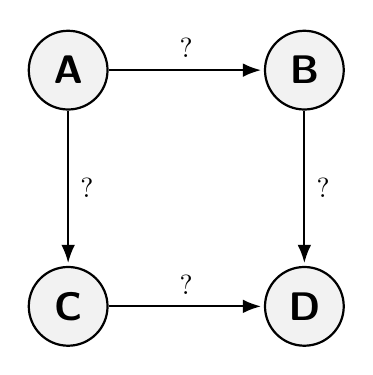
\begin{tikzpicture}[->,>=Latex,shorten >=1pt,auto,node distance=3cm,
  thick,main node/.style={circle,fill=gray!10,draw,
  font=\sffamily\Large\bfseries,minimum size=10mm}]

  \node[main node] (a) {A};
  \node[main node] (b) [right of=a] {B};
  \node[main node] (c) [below of=a] {C};
  \node[main node] (d) [right of=c] {D};

  \path[every node/.style={fill=white,inner sep=4pt}]
  % replace '?' with your own edge weight below
    (a) edge [] node[] {$?$} (b)  % edit this line
    (a) edge [] node[] {$?$} (c)  % edit this line
    (b) edge [] node[] {$?$} (d)  % edit this line
    (c) edge [] node[] {$?$} (d); % edit this line
\end{tikzpicture}}
\end{center}

 After assigning edge weights in the graph above, which path would Dijkstra's algorithm choose, and what is the length of that path?
 
\solution{
% your solution here
}

\vskip 2em
 Which path is actually the shortest path, and what is the length of that path?
 
\solution{
% your solution here
}

\vskip 2em


%%%%%%%%%%%%%%%%%%%%%%%%%%%%%%%%%%%%%%%%%%%%%%%%%%%%%%%%

\begin{problem} Ancient Population Study \end{problem}
Historians are studying the population of the ancient civilization of \textit{Algorithmica}.  Unfortunately, they have only uncovered incomplete information about the people who lived there during Algorithmica's most important century. While they do not have the exact year of birth or year of death for these people, they have a large number of possible facts from ancient records that say when a person lived relative to when another person lived. 

These possible facts fall into two forms: 
\begin{itemize}
    \item The first states that one person died before the another person was born.
    \item The second states that their life spans overlapped, at least partially. 
\end{itemize} 

The Algorithmica historians need your help to answer the following questions. First, is the large collection of uncovered possible facts internally consistent? This means that a set of people could have lived with birth and death years that are consistent with all the possible facts they've uncovered. (The ancient records \textit{may not be accurate}, meaning all the facts taken together cannot possibly be true.) Second, if the facts are consistent, find a sequence of birth and death years for all the people in the set such that all the facts simultaneously hold. (Examples are given below.)

We'll denote the $n$ people as  $P_1, P_2,\ldots, P_n$. For each person $P_i$, their birth-year will be $b_i$ and their death-year will be $d_i$.  (Again, for this problem we do not know and cannot find the exact numeric year value for these.)

The possible facts (input) for this problem will be a list of relationships between two people, in one of two forms:
\begin{itemize}
\item $P_i \textit{ prec } P_j$ (indicates $P_i$ died before $P_j$ was born)
\item $P_i \textit{ overlaps } P_j$ (indicates their life spans overlapped)
\end{itemize}

If this list of possible facts is not consistent, your algorithm will return ``not consistent''.  Otherwise, it will return a possible sequence of birth and death years that is consistent with these facts.

Here are some examples:
\begin{itemize}

\item The following facts about $n=3$ people are \textbf{not} consistent: 
$P_1 \textit{ prec } P_2$. 
$P_2 \textit{ prec } P_3$. 
$P_3 \textit{ prec } P_1$.

\item The following facts about $n=3$ people \textbf{are} consistent: 
$P_1 \textit{ prec } P_2$ and $P_2 \textit{ overlaps } P_3$. Here are two possible sequences of birth and death years:

\hspace*{2em} $b_1, d_1, b_2, b_3, d_2, d_3$ \\
\hspace*{2em} $b_1, d_1, b_3, b_2, d_2, d_3$ \\
(Your solution only needs to find one of any of the possible sequences.)
\end{itemize}

\textbf{Your answer should include the following.} Clearly and precisely explain the graph you'll create to solve this problem, including what will form the nodes and edges. Explain how you'll use one or more of the algorithms we've studied to solve this graph problem, and explain why this leads to a correct answer. Finally, give the time-complexity of your solution.

\solution{
% your solution here
}

%%%%%%%%%%%%%%%%%%%%%%%%%%%%%%%%%%%%%%%%%%%%%%%%%%%%%%%%
\begin{problem} Halloween Party Game \end{problem}

Prof. Bloomfield is planning a neighborhood Halloween party and wants to create a fun game for the neighborhood kids that encourages them to work together. To setup his game, Prof. Bloomfield secretly counts out a certain number of candy bars and puts them in a large class jar. The rules are that each kid can only make one guess, and after that the children will be told that the guess is either: correct, too high, or too low. Assuming the guess is incorrect, another child can make a guess, and so on, until either the correct guess has been made or until every child has made a guess. If the correct number is guessed, the children get the candy bars to share. If each child has guesses incorrectly, Prof. Bloomfield will laugh maniacally and eat all of the candy bars in front of the children. 

The children look around and notice that there are only 10 children, but many times more candy bars, making the guessing almost impossible. The children are discouraged, thinking that Prof. Bloomfield has given them a game that is impossible to win. However, in a rare act of benevolence, Prof. Bloomfield tells them that there are no more than 100 candy bars in the jar, and that with 10 guessers they are assured of winning if they come up with a good guessing strategy and work as a team.
\vskip 2em

Clearly describe an algorithm that can be used to insure that the correct number is guessed within 10 guesses. 

\solution{
% Your solution here
}
\vskip 2em

Write out the recurrence relation for your algorithm in terms of $T(n)$. (Note: This may help you with formatting: $T(n)=aT(\frac{n}{b})+c$

\solution{
% Your solution here
}
\vskip 2em

State the asymptotic runtime of your algorithm.

\solution{
% Your solution here
}
%%%%%%%%%%%%%%%%%%%%%%%%%%%%%%%%%%%%%%%%%%%%%%%%%%%%%%%%
\end{document}
